\documentclass[12pt,letterpaper,noanswers]{exam}
\usepackage[usenames,dvipsnames,svgnames,table]{xcolor}
\usepackage[margin=0.9in]{geometry}
\renewcommand{\familydefault}{\sfdefault}
\usepackage{multicol}
\pagestyle{head}
\header{AM 108 Class 16}{}{van der Pol}
\runningheadrule
\headrule
\usepackage{graphicx} % more modern
\usepackage{amsmath} 
\usepackage{amssymb} 
\usepackage{hyperref}
\usepackage{tcolorbox}

\begin{document}
 \pdfpageheight 11in 
  \pdfpagewidth 8.5in

\noindent 




\begin{itemize}
    \item Problem set 06 is due Friday October 16th.
    \item There is not a pre-class assignment for Friday.
    \item There will be a skill check in class on Friday.  The problem info is below.
    \item There is a quiz on Monday October 19th.  I will be available on Slack/APMTH 108 Zoom from 1pm-2:30pm on Monday to answer questions that arise as you take the quiz.
\end{itemize}

\hrule
\vspace{0.2cm}



\noindent\textbf{Teams}

\begin{multicols}{2}
1. 
\end{multicols}

\noindent \textbf{Teams 1 and 2}: Post screenshots of your work to the course Google Drive today.  Include words, labels, and other short notes that might make those solutions useful to you or your classmates.  Find the link in Canvas (or here: \url{https://drive.google.com/drive/u/0/folders/1GcpwvKHD4tMecpFQ4lNxN_r5Ylj7YHbd})

\vspace{0.2cm}

\hrule
\vspace{0.2cm}

\noindent\textbf{Big picture}

We have been working on how to construct a phase portrait for a 2d system in $\mathbb{R}^2.$ Recently we have been trying to determine whether or where a phase portrait might have closed trajectories.  

Today we are looking at a single important example of a system that has a limit cycle (an isolated closed trajectory).  This example system is called the van der Pol oscillator.


\vspace{0.2cm}
\hrule
\vspace{0.2cm}


\noindent \textbf{Extra vocabulary / extra facts:}
\begin{tcolorbox}
Definitions and examples are from \underline{Noise-Induced Phenomena in Slow-Fast Dynamical Systems:} \underline{A Sample-Paths Approach} by Berglund and Gentz.  Springer.  2006.

We have encountered a \textbf{rate parameter} in many dynamical systems.  Such a parameter has a dimension of $\frac{1}{T}$.  

A rate parameter often sets a \textbf{timescale}, such as the relaxation time towards an equilibrium or the period of a periodic orbit.  Such a timescale would be related to the inverse of the rate parameter (and has a dimension of $T$).  For example, in the linear system $\dot x = a x$ with solutions $x(t) = x_0e^{at}$, the size of $x$ changes by a factor of $2$ when $e^{at} = 2$ so when $t = \frac{1}{a}\ln 2$.  $\frac{1}{a}$ is a timescale that is being set by the rate parameter $a$.

In a dynamical system with two timescales, it is possible for the timescales to be well-separated.  In a predator-prey system, timescale separation could happen if the prey reproduces quickly and the predators reproduce slowly.  In a desert ecosystem, this could happen if rain events were short and water flowed through the ecosystem quickly, while biological activity occurred more slowly.  A \textbf{separation of timescales} allows us to write a dynamical system as a \textbf{slow-fast ODE}.
\end{tcolorbox}
\begin{tcolorbox}
In a system with two timescales, $t$ and $s$ with $s = \epsilon t $ for $\epsilon$ small, where $t$ is the fast timescale, and $s$ is the slow timescale, a separation of timescales often allows us to write the system in slow time as $\displaystyle\left\{\begin{array}{c} \epsilon \frac{dx_s}{ds} = f(x_s,y_s) \\ \frac{dy_s}{ds} = g(x_s,y_s) \end{array}\right.$ or in \textbf{fast time} as $\displaystyle\left\{\begin{array}{c} \frac{dx_t}{dt} = f(x_t,y_t) \\ \frac{dy_t}{dt} = \epsilon g(x_t,y_t) \end{array}\right.$

A \textbf{relaxation oscillation} is a periodic motion in which fast and slow phases alternate.

After being rewritten via a Lienard transformation, the \textbf{van der Pol} oscillator system can be written as $\displaystyle\left\{\begin{array}{c} \frac{dx_t}{dt} = \mu(y-F(x)) \\ \frac{dy_t}{dt} = \frac{1}{\mu} (-x) \end{array}\right.$.  When $\mu \gg 1$ then $\frac{1}{\mu}$ is small, and this is an example of a slow-fast ODE written in fast time.
\end{tcolorbox}
\begin{tcolorbox}
A dynamical system is called \textbf{weakly nonlinear} when the system is a small perturbation away from a linear system.  

In its weakly nonlinear form, the van der Pol system can be written as $\ddot x + x + \epsilon \dot x(x^2-1) = 0$ where $\epsilon$ is a small parameter.  This is a \textbf{small perturbation} from the system $\ddot x + x = 0$, which is a conservative system ($E(x,\dot x) = \frac{1}{2}x^2 + \frac{1}{2}\dot x^2$ is conserved) and has solutions of the form $x(t) = A\cos t + B\sin t$ (for arbitrary $A$ and $B$).

The presence of the $\epsilon \dot x (x^2-1)$ term changes the vector field only very slightly from the vector field in the system $\ddot x + x = 0$.

We can use an \textbf{energy method} for approximating the location of a limit cycle in the weakly nonlinear system.  On a limit cycle, we move periodically in phase space, so $E(x,\dot x)$ will also have to be periodic.  Look at $\Delta E$ over one cycle.  This will be $0$ on a limit cycle, so to approximate the limit cycle, find a trajectory over which $\Delta E = 0$.
\end{tcolorbox}



\vspace{0.2cm}
\hrule
\vspace{0.2cm}

\noindent\textbf{Your Questions}
\begin{enumerate}
    \item Steve says he uses the Lienard transformation so that the limit cycle will tend to a constant shape.  What does he mean?
    
    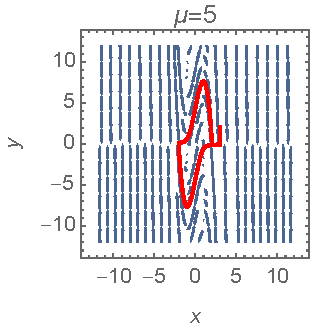
\includegraphics{img/C16vdp-p1a.pdf}
     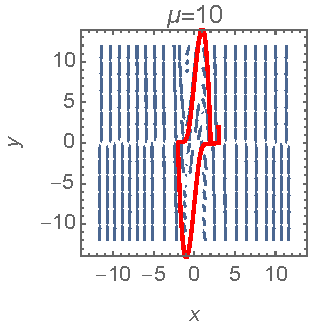
\includegraphics{img/C16vdp-p1b.pdf}\hfill
      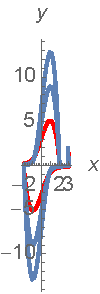
\includegraphics{img/C16vdp-p1c.pdf}
      
\item Drawing the limit cycle
\begin{enumerate}
    \item Why does the initial point move right until it reaches the nullcline?  How do we find the limit cycle shape?

\item Why doesn't the trajectory go above the cubic curve?

\item How do we know the trajectory stays ``outside'' the nullcline?
\end{enumerate}



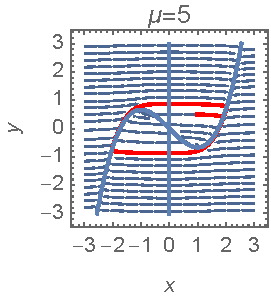
\includegraphics[width=2in]{img/C16vdp-p2a.pdf}
     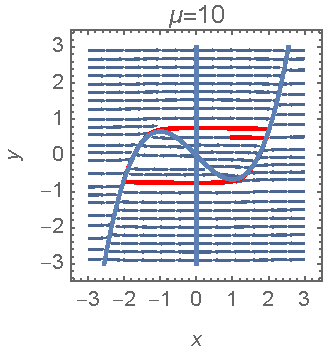
\includegraphics[width=2in]{img/C16vdp-p2b.pdf}\hfill
      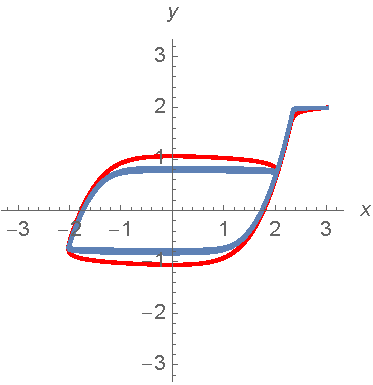
\includegraphics{img/C16vdp-p2c.pdf}

\item In the new rescaled system, $\dot x$ and $\dot y$ each depend on $\mu$.  How does that lead to a limit cycle that is unique for each $\mu$?

\item In the change of variables process, how do we return to $x$ and $y$ after the transformation?  Can we use this change of variables for other systems?

\item How did we know to use this transformation?  Can we use similar methods for other problems?

\item What is special about this system?  

\item Why do we limit our analysis to large $\mu$ and to small $\mu$?  What happens at intermediate $\mu$?

\end{enumerate}


\vspace{0.2cm}
\hrule
\vspace{0.2cm}

\noindent\textbf{Skill Check C17 practice}
\begin{questions}
\item Retake of skill check C14: index theory.

\item Set up an integral in a single variable for the amount of time it takes a trajectory to traverse the curve $y = F(x)$ from $x = x_0$ to $x = x_1$, when $\dot y = g(x) = x$.

\vspace{0.2cm}

\hrule
\vspace{0.2cm}
\end{questions}



\noindent\textbf{Skill check C17 practice solution}


$\displaystyle T = \int_{x_0}^{x_1} \dfrac{dt}{dy}\dfrac{dy}{dx}dx$ 

$y = F(x)$ on our trajectory so we have $\frac{dy}{dx} = F'(x)$ on our trajectory.

Using $\frac{dt}{dy} = 1/\dot y$, we have
$\displaystyle T = \int_{x_0}^{x_1} \frac{1}{x}F'(x)dx$.


\vspace{0.2cm}
\hrule
\vspace{0.2cm}





\eject



\vspace{0.2cm}

\hrule
\vspace{0.2cm}

\noindent \ \ 0.  Introduce yourself to your new team (and write your names on the slide).

\begin{questions}

\item (convince yourself of the details: van der Pol example) After a change of variables the van der Pol system is
\begin{align*}
\dot{x} = &\  \mu(y-\frac{1}{3}x^3 + x) \\
\dot{y} = &\ -\frac{1}{\mu} x.
\end{align*}
Consider the case where $\mu>>1$.
\begin{parts}
\item In this relaxation oscillation, the trajectory is moving very quickly when it jumps between the two parts of the $\dot{x}=0$ nullcline.
Using the $\dot{x}$ equation, convince yourself that it is moving at a velocity of $c\mu$, where $c$ is between $0.1$ and $2$ for most of the jump.  

\emph{On the plot below, a single trajectory is shown in red.  The $\dot x = 0$ nullcline is drawn with a solid black line.  The dashed lines are the curves $y - x^3/3 + x = \pm 0.1$ and the dotted lines are the curves $y - x^3/3 + x = \pm 1.4$.}


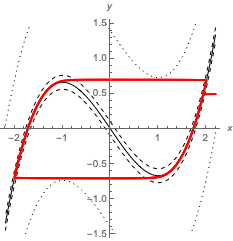
\includegraphics{img/191016-C17p3.png}

\emph{We sometimes say this velocity is of the order of $\mu$, or is $\mathcal{O}(\mu)$, because it is bounded above by a constant multiple of $\mu$.}

\item The trajectory is traversing a
distance of about $3$ as it jumps.  Combine the approximate distance and the approximate velocity to find the $\mu$-dependence of the time that it spends jumping.
%\item How close does the trajectory need to be to the $\dot{x} = 0$ 
% nullcline for both $\dot{x}$ and $\dot{y}$ to be the same order of magnitude?
\item While moving along the nullcline, the trajectory moves about $1$ unit in $x$ and a bit less than $2$ units in $y$.  It is basically moving along the curve
$y = \frac{1}{3}x^3-x$ (it is not quite on the curve, but it is close to that curve the whole time).  The time it spends 
traversing the curve is a constant multiple of $\mu^k$ for some integer $k$.  


To estimate time (just as we did for the oscillators in chapter 4), we set up an integral of the form $\displaystyle\int_{x_1}^{x_2} \frac{dt}{dx}dx$
or something like this.  This integral shows us how the time depends on $\mu$.  Using  \[\int_{x_1}^{x_2} \frac{dt}{dx}dx\]
doesn't work so well.  It
puts $y-(\frac{1}{3}x^3-x)$ in the denominator (so a dependence on $x$ and $y$, not just $x$).
What is wrong with having a dependence on $x$ and on $y$ in the integral?

\item We could try again with \[\int_{y_1}^{y_2} \frac{dt}{dy}dy.\]  Argue that this leads to a problem, too, and isn't something we can integrate.

\item 
So actually, Steve used \[\int_{x_1}^{x_2} \frac{dt}{dy}\frac{dy}{dx}dx.\]  
(This is an example of persisting until something works, and luckily getting something to work before we run out of options).  Confirm that this expression results in something that is integrable.

\emph{Note that for $\frac{dy}{dx}$ we're thinking of ourselves as, to good approximation, being
stuck on the nullcline, so compute this directly by assuming the trajectory is exactly on the nullcline.}

\item
Use the setup of this final integral to identify $k$.  There is no need to evaluate the integral.  We just want to learn the $\mu$ dependence of the time.  
\item Compare the amount of time spent jumping to the amount of time spend moving along the curve.  (We have the timescales
of these processes, and not the exact amounts of time, so compare the timescales).
\end{parts}


  
\question (weakly nonlinear van der Pol) Let $E(x,\dot x) = \frac{1}{2}x^2+\frac{1}{2}\dot x^2$.
\begin{parts}
\part Find $\frac{dE}{dt}$ for the weakly nonlinear van der Pol oscillator, where $x+\ddot x = -\epsilon \dot x (x^2-1)$.

\emph{Write $\dot E$ in terms of just $x$ and $\dot x$.}

\part We have $\Delta E = \int_0^T \frac{dE}{dt}dt$.  The weakly nonlinear van der Pol is very close to the system $\ddot x + x = 0$.  Two trajectories are shown for each system in the plots below.

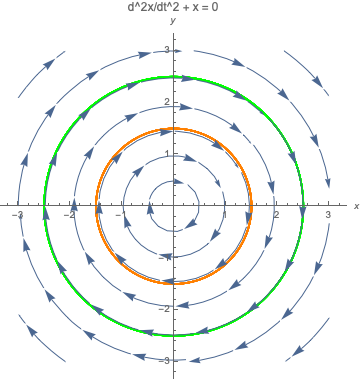
\includegraphics[width=3in]{img/191016-C17p1.png}
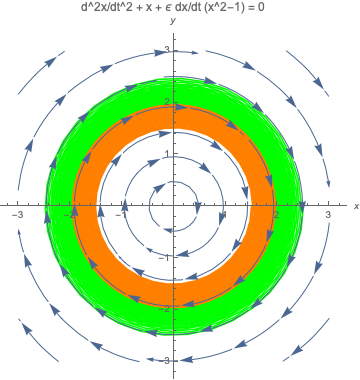
\includegraphics[width=3in]{img/191016-C17p2.png}

In the $\ddot x + x = 0$ system, the period of cycles is $T = 2\pi$, and $x(t) = A\cos t$ is a solution for any $A$.  In the weakly nonlinear van der Pol system, assume there exists a limit cycle (we know that there is one from Lienard's theorem), and that it is of the form $x(t) = A\cos t$ with period $T\approx 2\pi$.  We want to find the value of $A$ associated with the limit cycle.
\begin{itemize}
    \item Find $\dot x$ assuming $x(t) = A\cos t$.
    \item Substitute $\dot x$ and $x$ into 

$\Delta E \approx -\epsilon \int_0^{2\pi} \dot x^2 (x^2-1) dt$

\item  Using $\displaystyle \frac{1}{2\pi} \int_0^{2\pi} \sin^2 t dt = \frac{1}{2}$ and $\displaystyle \frac{1}{2\pi}\int_0^{2\pi} \cos^2 t\sin^2 t dt = \frac{1}{8}$, find a value of $A$ such that $\Delta E = 0$.
\item Check the $A$ you found against what is happening in the phase portrait above.
\end{itemize}




\end{parts}

% \item (Time averaging an oscillation over a single period) Show the time averaging facts that you used above.

% Find $\left<(\sin t)^2\right>$ or $\left<(\cos t)^2(\sin t)^2\right>,$ where $\left< f \right>$ denotes the average of a periodic function $f$ over a single cycle.  For $f(t)$ a function of period $2\pi$, we can compute this average as $\frac{1}{2\pi}\int_0^{2\pi}f(t)dt$.

% I find that a straightforward way to compute this type of quantity is to use $\cos t = \frac{1}{2}(e^{it}+e^{-it})$ and $\sin t = \frac{1}{2i}(e^{it}-e^{-it})$.  

% Note that $\cos nt = \frac{1}{2}(e^{int}+e^{-int}$.  Also note that $\int_0^{2\pi} \cos nt\ dt =0$ for $n=1,2,3,...$.

\end{questions}

\eject

\textbf{Answers:}

\begin{enumerate}
\item
\begin{enumerate}
\item When the trajectory is flowing across, $\dot{y}$ is small: $\vert x \vert < 3$ or so, and $\mu$ is big, so $\vert \frac{x}{\mu} \vert < \frac{3}{\mu}$, which is small
(specifically order of $\frac{1}{\mu}$.  
This means the motion is basically horizontal.  And it is moving at a speed of $\mu (y-x^3/3 + x)$ in the horizontal direction.
Away from the nullcline itself, $y-x^3/3 + x$ is between $0.1$ and $1.4$ for almost the whole distance across, so $\dot x$ will be between $0.1\mu$ and $1.4\mu$ for most of the jump.
\item It jumps across a distance of maybe $3$ as it
moves horizontally.
Since $distance/time = velocity$ the time is $distance/velocity$, so it is proportional to $\frac{1}{\mu}$.  This will be very small and means that it jumps across pretty quickly.
%\item For $\dot{x}$ and $\dot{y}$ to be the same order we need them to both be order $\frac{1}{\mu}$ so we need $(y- x^3/3 + x)$ to be
%order $\frac{1}{\mu^2}$ so that when it is multiplied by $\mu$ it is order $\frac{1}{\mu}$.  So we need to be within order $\frac{1}{\mu^2}$ of the
% nullcline.
\item Along the nullcline, $x$ and $y$ each depend on $t$, but they also have a relationship with each other.  The integral $\int_{x_1}^{x_2} \frac{1}{y+x-x^3/3}dx$ isn't something that we can integrate because $y$ is coupled to $x$ as we move along the nullcline, so we can't treat $y$ as a constant while we integrate with respect to $x$.  Instead, we would need to write $y$ in terms of $x$.
\item This one is $\int_{y_1}^{y_2} -\frac{\mu}{x}dy$ so also mixes together $x$ and $y$.  As $y$ changes, $x$ also changes, so we can't integrate this without knowing how they relate to each other.  Instead, we would need to write $x$ in terms of $y$.
\item On the nullcline, $y = -x+x^3/3$ so $\frac{dy}{dx} = -1 + x^2$.  $\displaystyle \int_{x_1}^{x_2} -\frac{\mu}{x}(x^2-1)dx$.  This is an integral where the integrand doesn't depend on $y$ or $t$ but just on $x$, and it is being integrated $dx$, so this one can be computed as written.
\item $\frac{dt}{dy} = -\mu\frac{1}{x}$ and $\frac{dy}{dx} = x^2 - 1$ on the nullcline.  So $\displaystyle T = \int_{x_1}^{x_2} -\mu \frac{1}{x}(x^2-1) dx = \mu\int_{x_1}^{x_2} - \frac{1}{x}(x^2-1) dx.$
This is $\mu$ multiplied by a constant that doesn't depend on $\mu$.  So this time is proportional to $\mu$ meaning that $k = 1$.
\item The jump is order of $\frac{1}{\mu}$ and the motion along the curve is order of $\mu$.  This means we spend a ton more time on the 
curve compared to doing the jump.
\end{enumerate}

\item \begin{enumerate}
    \item 
 $\dot E = x \dot x + \dot x \ddot x = \dot x(x + \ddot x) = -\epsilon \dot x^2(x^2-1)$
 \item $\dot x = -A \sin t$.  $\Delta E = -\epsilon \int_0^{2\pi}A^2\sin^2 t(A^2\cos^2 t - 1)dt = -\epsilon\left(A^4/8 -A^2/2\right)$.  $A^4/8 - A^2/2 = 0$ so $A^2/4  = 1 \Rightarrow A = 2$.  This looks like it matches the location where the green trajectory and the orange trajectory touch.  If the orange one is moving outward and the green one inward, then there is a limit cycle at about $A \approx 2$.
 \end{enumerate}
% \item $\frac{1}{2}$ and $\frac{1}{8}$.
\end{enumerate}

\end{document}